\begin{frame}
\frametitle{Mixture models: obtaining the a posteriori probabilities}
\begin{itemize}
\item A sample $X= \{\textbf{x}_1, \dots, \textbf{x}_i, \dots, \textbf{x}_n\}$.
\item<2-> A fitted mixture model with $k$ components $C_j$, $1 \leq j \leq k$.
\item<3-> $\tau_{ij} = P( \left\{ \textbf{x}_i \in C_j \right\})$, $1 \leq i \leq n$ and $1 \leq j \leq k$.
\end{itemize}
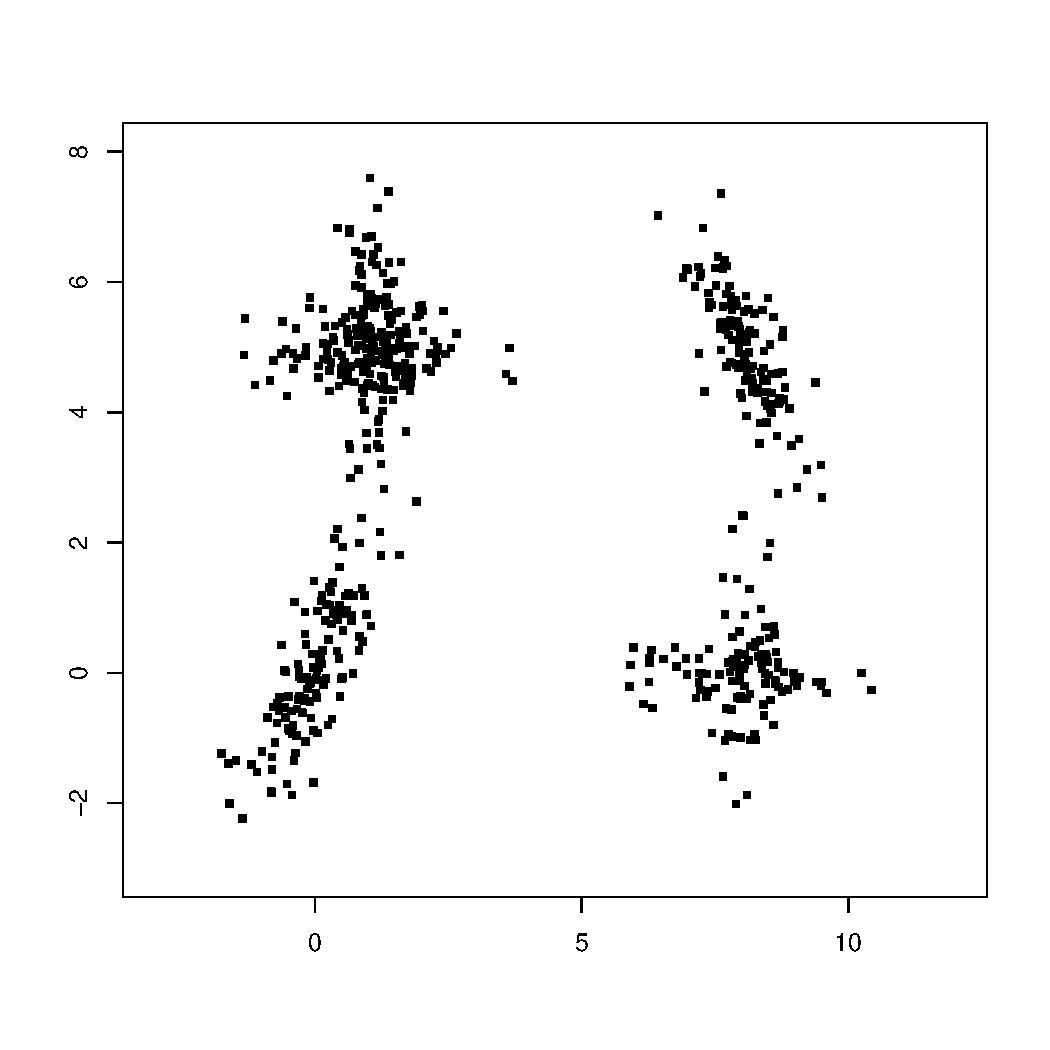
\includegraphics[width=0.33\textwidth]{data41.pdf}
\visible<2->{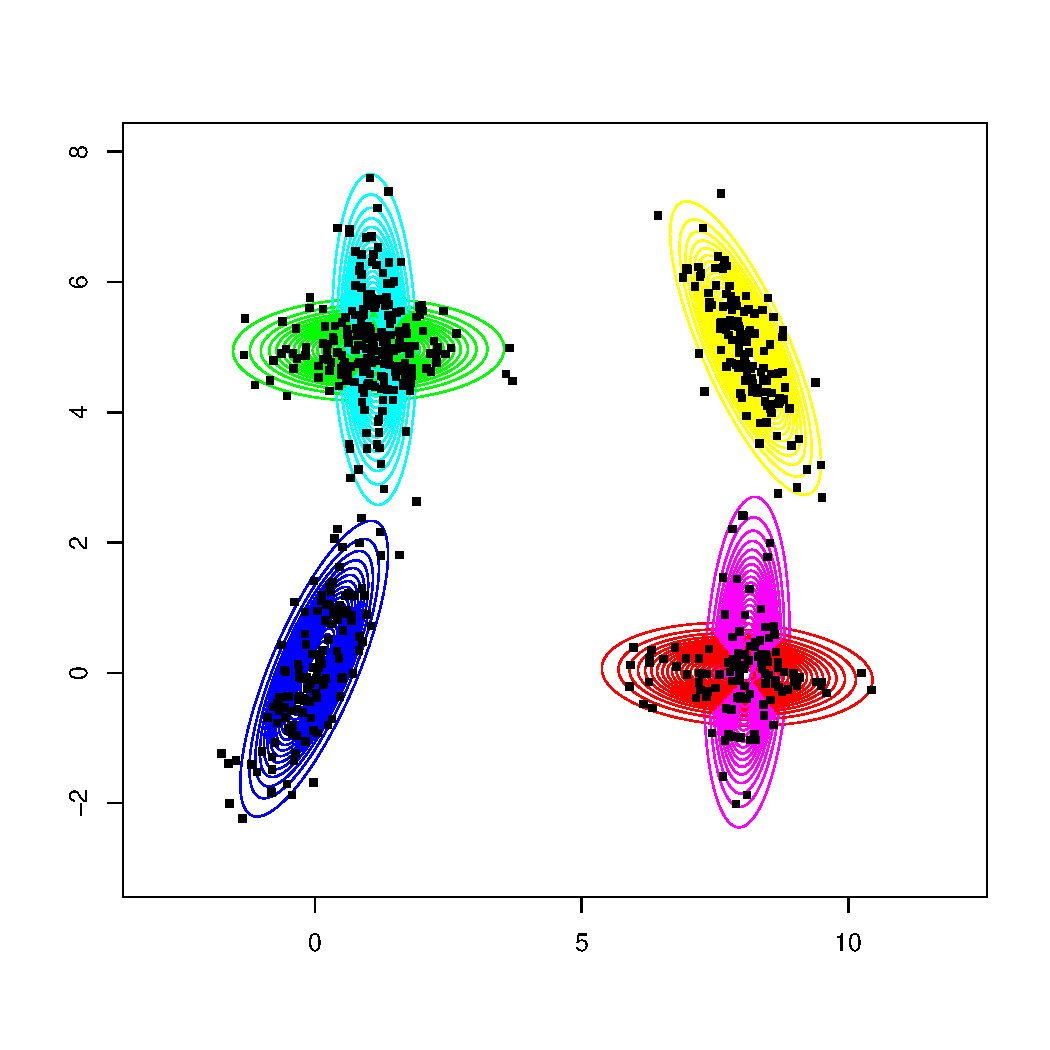
\includegraphics[width=0.33\textwidth]{data41dist.pdf}}
\visible<3->{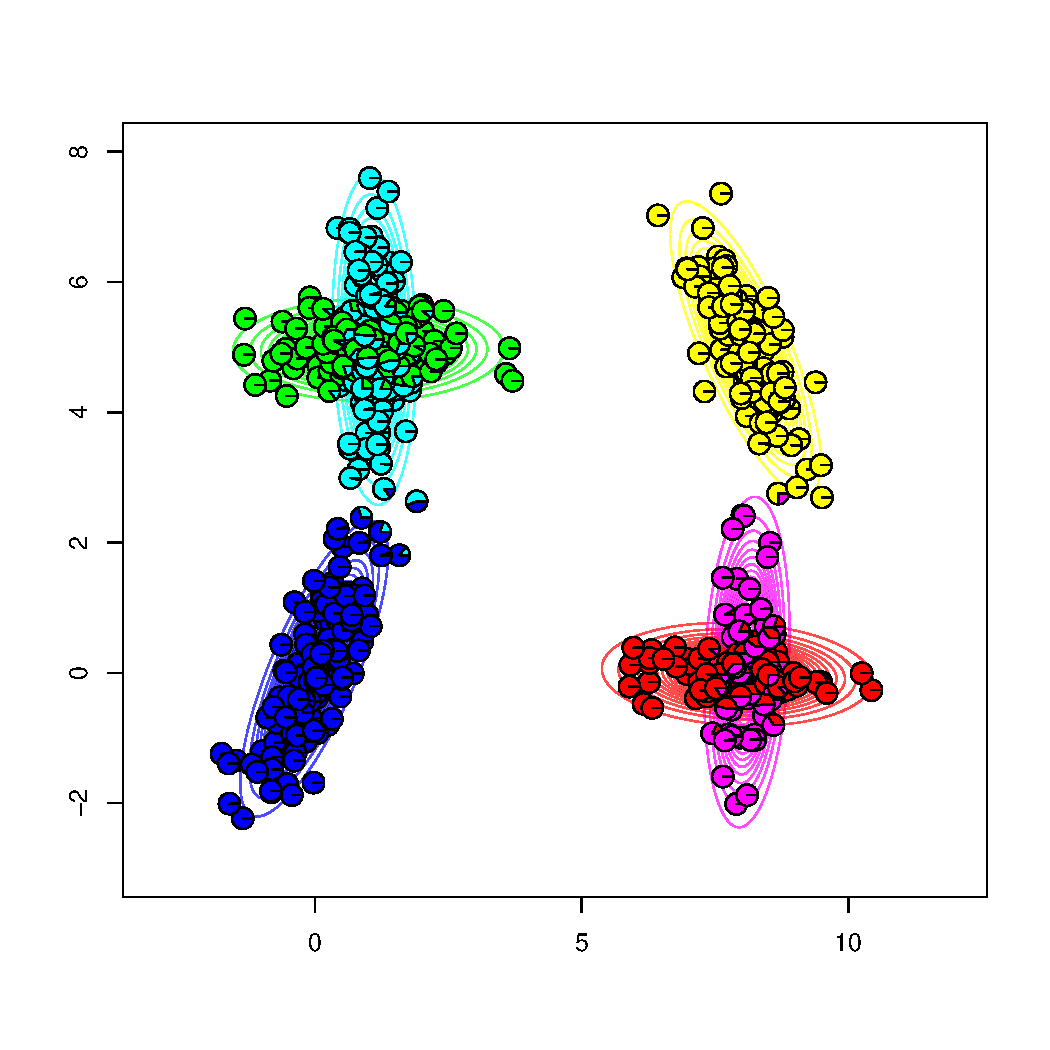
\includegraphics[width=0.33\textwidth]{data41posteriori.pdf}}
\end{frame}

\begin{frame}[t]
\frametitle{Whats does "merge" usually mean  in mixture modeling?}
\begin{itemize}
\item Merging class $C_a$ with class $C_b$ to a new class $C_c$ means that observation related to class $C_{ab}$ either is related to class $C_a$ or to class $C_b$.
\item Mixture models assume that an observation comes from a unique component (belongs to a unique class).
\item For an observation $\textbf{x}_i$ 
\begin{eqnarray*} 
\uncover<2>{ \tau_{i c}  \;=\;} P( \{ \textbf{x}_i \in C_{c} \})  &=& P( \{ \textbf{x}_i \in C_{a} \} \cup \{ \textbf{x}_i \in C_{b} \} ) \\
&=& P( \{ \textbf{x}_i \in C_{a} \}) + P( \{ \textbf{x}_i \in C_{b} \} )  \uncover<2>{ \;=\; \tau_{i a} + \tau_{i b} }
\end{eqnarray*} 
\end{itemize}
\end{frame}

\begin{frame}[t]
\frametitle{Entropy approach}
\begin{block}{Entropy approach (Baudry et~al., 2010)}
The classes to be merged are those that maximize the entropy of a posteriori probabilities
\end{block}
\small
\only<1-2>{
\uncover<2>{Maximize}
\[
\overbrace{ 
\uncover<2>{-\left(} \sum_{i=1}^n \left\{ \tau_{iI_a} \log(\tau_{iI_a}) + \tau_{iI_b} \log(\tau_{iI_b})\right\} + \sum_{i=1}^n \sum_{\substack{\ell = 1\\\ell \neq a,b}}^k  \tau_{iI_\ell} \log(\tau_{iI_\ell}) \uncover<2>{\right)+}
}^{
\substack{\text{entropy }\\\text{before merging}}  
} 
\]
\[
\underbrace{ 
\uncover<2>{+\left( } \sum_{i=1}^n  (\tau_{iI_a}+\tau_{iI_b}) \log(\tau_{iI_a} + \tau_{iI_b}) + \sum_{i=1}^n  \sum_{\substack{\ell = 1\\\ell \neq a,b}}^k  \tau_{iI_\ell} \log(\tau_{iI_\ell}) \uncover<2>{\right)}
}_{
\substack{\text{entropy }\\\text{after merging}}   
} 
\]
}
\only<3>{
Maximize
\[
- \sum_{i=1}^n \left\{ \tau_{iI_a} \log(\tau_{iI_a}) + \tau_{iI_b} \log(\tau_{iI_b})\right\} + \sum_{i=1}^n  (\tau_{iI_a}+\tau_{iI_b}) \log(\tau_{iI_a} + \tau_{iI_b})
\]
}
%\only<4>{
%Minimize
%\[
% \sum_{i=1}^n \left\{ \tau_{iI_a} \log(\tau_{iI_a}) + \tau_{iI_b} \log(\tau_{iI_b})\right\} - \sum_{i=1}^n  (\tau_{iI_a}+\tau_{iI_b}) \log(\tau_{iI_a} + \tau_{iI_b})
%\]
%}
\end{frame}

\begin{frame}
\frametitle{Summarizing}

\begin{itemize}
\item How to combine?
\begin{itemize}
\item Amalgamation:
\item Geometric mean: ${\boldsymbol\tau}^{\mathcal{I}}_i$
\end{itemize}
\item How to evaluate the combination of $a$and $b$?
\[ \frac{  
  \mathlarger\sum_{i=1}^n
		\omega ({\boldsymbol\tau}^{\mathcal{I}}_i, a) \cdot
		\theta ({\boldsymbol\tau}^{\mathcal{I}}_i, a, b)
}{  
	\mathlarger\sum_{i=1}^n  
		\omega ({\boldsymbol\tau}^{\mathcal{I}}_i, a) 
}, \]
\end{itemize}
\end{frame}

\begin{frame}
\frametitle{Methods}
\begin{itemize}
\item Methods based on modality
\begin{itemize}
\item The ridgeline unimodal method
\end{itemize}
\item Methods based on misclafication probabilities
\begin{itemize}
\item Bhattacharyya distance method
\item Entropy approach
\item Directly estimated misclassification probabilities
\end{itemize}
\end{itemize}
\end{frame}


\begin{frame}
\frametitle{Entropy approach}
\end{frame}

\begin{frame}
\frametitle{Directly estimated misclassification \\probabilities (DEMP)}
\end{frame}
